\documentclass[11pt]{article}
\usepackage[margin=1in]{geometry}
\usepackage{amsmath}
\usepackage{booktabs}
\usepackage{graphicx}
\usepackage{hyperref}
\usepackage{microtype}
\usepackage{xcolor}
\usepackage{tikz}
\usetikzlibrary{arrows.meta,positioning}

\definecolor{ink}{HTML}{172033}
\definecolor{accent}{HTML}{0B5C6B}
\hypersetup{colorlinks=true,linkcolor=accent,citecolor=accent,urlcolor=accent,
  pdftitle={A Reproducible Event-Sourcing and Process-Mining Workpack for Freedom-of-Information Records},
  pdfauthor={Dylan A. Mordaunt}}
\urlstyle{same}
\emergencystretch=2.5em
\setlength{\parskip}{0.25em}
\setlength{\parindent}{1.15em}
\renewcommand{\arraystretch}{1.12}

\title{A Reproducible Event-Sourcing and Process-Mining Workpack for Freedom-of-Information Records}
\author{Dylan A. Mordaunt\\\small Independent researcher\\\small \href{https://orcid.org/0000-0002-9775-0603}{ORCID: 0000-0002-9775-0603}}
\date{Version 0.1.0, July 2026}

\begin{document}
\maketitle

\begin{abstract}
Freedom-of-information archives contain process traces, revisions, attachments, and decisions, but
these materials are difficult to analyse reproducibly when capture, legal semantics, document
extraction, and process mining are mixed together. This paper presents \texttt{foi-process}, an
open-source Rust workpack that treats archive snapshots and future live deltas as one deterministic
event stream. The implementation provides typed identifiers, RFC 8785 canonical content IDs,
revision-aware replay, correction and retraction handling, portable OCEL projections, an optional
Rust4PM adapter, privacy-aware public projections, and checksummed publication bundles. Synthetic
scale evidence covers 1,000, 10,000, and 200,000 cases, with one million baseline events in the
largest profile. The largest profile completed in 8.45 seconds on the recorded Windows host and
used at most 814.4 MB of resident memory. These measurements are engineering evidence, not a
claim about live archive performance. The repository publishes derived event logs and a dashboard
separately from the software release, retains source-specific rights for archive material, and
fails closed when governance conditions for public data are not met.
\end{abstract}

\section{Introduction}
Public freedom-of-information systems expose more than individual documents. They also expose
requests, acknowledgements, transfers, extensions, decisions, releases, refusals, and later
corrections. Those records can support process analysis, but only if an analysis preserves the
difference between an observed source record, a revised interpretation, a legal classification,
and a derived process statistic. Treating these as ordinary rows makes replay, correction, and
provenance errors hard to detect.

\texttt{foi-process} is a software and data-publication workpack for this problem. It is designed
around the repository boundary that capture belongs to \texttt{fyi-cli}, immutable snapshots and
mirrors belong to \texttt{fyi-archive}, legal vocabulary belongs to \texttt{foi-o}, and generic
process-mining algorithms belong to Rust4PM. The workpack supplies the integration, replay, and
public-projection layer between those systems \cite{foi-cli,foi-archive,foi-o,rust4pm}.

The contribution is an auditable event spine rather than a new process-mining algorithm. It makes
logical event identity independent of mutable activity labels, represents corrections and
retractions as revisions, preserves source order separately from event time, and packages the
result with manifests and byte-level digests. The accompanying dashboard and Hugging Face Dataset
are publication surfaces for derived public-safe outputs, not substitutes for the source archive.

\section{Design requirements}
The design follows five requirements.
\begin{enumerate}
  \item A source record must remain traceable through normalisation, replay, projection, and
    publication without exposing private source material.
  \item A correction must update the logical event it corrects rather than create a second event
    merely because its activity label changed.
  \item Archive snapshots and live continuations must use the same delta and replay semantics.
  \item Public projections must be conservative: text, OCR, embeddings, and sensitive metadata are
    withheld unless the publication disposition permits them.
  \item Every derived deposit must be reproducible from a named revision, manifest, and checksum;
    a successful workflow alone is not treated as publication evidence.
\end{enumerate}

\section{System design}
\subsection{Event and evidence model}
The event spine separates evidence records, object records, event records, object links, and
revision metadata. Events refer to evidence rather than embedding full documents in every row.
Each logical event has a stable identity derived from canonical content and an explicit revision
history. Activity names are attributes of a revision, not part of the identity of the underlying
logical event. This distinction prevents a label correction from silently changing counts or
creating a duplicate case transition.

Canonical identifiers use JSON Canonicalization Scheme (JCS), which provides deterministic bytes
for cross-language hashing \cite{rfc8785}. SHA-256 digests are recorded for source attachments,
archive containers, generated artefacts, and publication manifests. Byte length is recorded with
digests so that verification checks both content and the expected file boundary.

\subsection{Replay and live continuation}
Archive snapshots are converted to ordered deltas. A live continuation appends deltas to the same
normaliser and replay engine. The replay layer detects duplicate revisions, stale revisions,
revision gaps, stream-position gaps, position regressions, conflicts, corrections, and
retractions. Checkpoints include state hashes and are committed after durable output state. A
restored snapshot is rejected when its state hash or record partition does not match the recorded
manifest.

Source order and event time are retained as different fields. Source order is used for replay and
deterministic dashboard calculations; timestamps are used for temporal views and may be absent,
coarse, or corrected. This prevents sorting a corrected event stream solely by display time.

\subsection{Process-mining boundary}
The workpack emits a portable OCEL-shaped projection and provides an optional adapter to the
existing Rust4PM \texttt{AppendableOCEL} interface. Rust4PM remains the canonical implementation
for generic process-mining algorithms. Local edges, variants, conformance findings, and dashboard
roll-ups are transport and publication projections; they are not presented as a replacement for
the upstream mining library \cite{ocel2,rust4pm}.

\begin{figure}[ht]
\centering
\resizebox{\linewidth}{!}{%
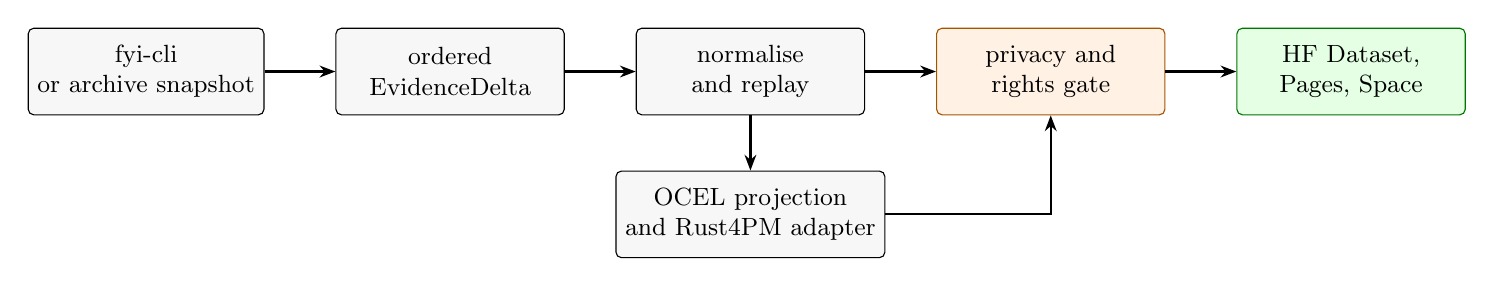
\begin{tikzpicture}[
  node distance=7mm and 9mm,
  box/.style={draw, rounded corners=2pt, align=center, minimum width=29mm, minimum height=11mm, font=\small, fill=gray!6},
  gate/.style={box, fill=orange!10, draw=orange!65!black},
  output/.style={box, fill=green!10, draw=green!45!black},
  arrow/.style={-{Stealth[length=2mm]}, thick}]
\node[box] (capture) {fyi-cli\\or archive snapshot};
\node[box, right=of capture] (delta) {ordered\\EvidenceDelta};
\node[box, right=of delta] (replay) {normalise\\and replay};
\node[gate, right=of replay] (privacy) {privacy and\\rights gate};
\node[output, right=of privacy] (deposit) {HF Dataset,\\Pages, Space};
\draw[arrow] (capture) -- (delta);
\draw[arrow] (delta) -- (replay);
\draw[arrow] (replay) -- (privacy);
\draw[arrow] (privacy) -- (deposit);
\node[box, below=of replay] (mining) {OCEL projection\\and Rust4PM adapter};
\draw[arrow] (replay) -- (mining);
\draw[arrow] (mining) -| (privacy);
\end{tikzpicture}
}
\caption{Publication-oriented architecture. Capture, replay, generic mining, and public
projection remain separate boundaries.}
\label{fig:architecture}
\end{figure}

\section{Implementation}
The implementation is a single Rust package with optional Rust4PM, Parquet, dataframe, and OCEL
storage features. Python scripts provide a reference pipeline, schema and governance checks, scale
suite, public dataset builder, dashboard projection builder, and release-evidence builder. The
repository also contains portable schemas, generated fixtures, replay journals, privacy review
records, and Conductor tracks linking implementation work to cross-repository promotion.

The public publication path is intentionally split. The Hugging Face Dataset contains derived event
logs, revision streams, OCEL tables, process edges and variants, conformance findings, dashboard
artefacts, and SHA-256 manifests. GitHub Pages and the free Hugging Face Space consume a verified
browser projection. The GitHub Release workflow stages Rust binaries, checksums, release evidence,
and build provenance as a draft. No Rust crate, paper, or paid service is published automatically.

\section{Evaluation}
\subsection{Deterministic correctness}
The test suite exercises duplicate, stale, conflicting, gapped, corrected, and retracted revisions;
checkpoint restoration; deterministic replay; RFC 8785 parity vectors; generated-schema checks;
public-output privacy validation; and dashboard projection consistency. These are contract tests,
not an evaluation against a representative live archive. A production continuation still requires
validation against a real WARC/WACZ and attachment sample.

\subsection{Synthetic scale evidence}
Table~\ref{tab:scale} reports the committed benchmark. Each profile has five events per case and
three repetitions. Stress runs add one correction every 20 logical events and one retraction every
1,000 events. The 200,000-case profile is a synthetic shape used to expose memory and replay costs;
it does not model the distribution of attachments, OCR, or archive I/O.

\begin{table}[ht]
\centering
\caption{Recorded synthetic scale evidence. Medians are from the baseline profile.}
\label{tab:scale}
\begin{tabular}{rrrrr}
\toprule
Cases & Baseline events & Time (s) & Throughput & Peak memory (MB)\\
\midrule
1,000 & 5,000 & 0.039 & 127,144/s & 9.3\\
10,000 & 50,000 & 0.390 & 128,069/s & 41.1\\
200,000 & 1,000,000 & 8.451 & 118,332/s & 814.4\\
\bottomrule
\end{tabular}
\end{table}

\section{Governance and publication boundaries}
The workpack does not infer legal entitlement, statutory compliance, or a public-interest
disposition from process data. FOI-O remains authoritative for legal semantics and jurisdictional
profiles. Source-derived records retain the rights, access conditions, removal pathways, and
provenance requirements of their source. The Apache-2.0 software licence does not relicense
archive records, attachments, or derived facts.

For a future non-public deployment, public identifiers must be replaced or wrapped by a
pseudonymised traceability mechanism with a separately controlled mapping. The public fixture
deposit uses synthetic reviewed records and metadata-safe projections. Production publication is
blocked until privacy, licensing, removal, threat-model, data-governance, live-archive, and
statutory-source reviews are complete.

\section{Limitations and next steps}
The current evidence does not establish full-corpus ingestion, representative live-archive
performance, OCR or embedding quality, transactional state-backend requirements, or OIA statutory
conformance. It also does not establish that the hosted dashboard ingests every record in the FYI
archive. The next engineering gates are a bounded real WARC/WACZ and attachment validation, live
\texttt{fyi-cli}/\texttt{fyi-archive} continuation, independent schema and JCS parity checks,
representative archive benchmarks, and a completed production governance review.

\section{Availability and declarations}
\textbf{Code and manuscript.} Source code and this manuscript are available at
\url{https://github.com/edithatogo/foi-process}. Repository code is licensed Apache-2.0. The
manuscript source package is intended for arXiv review and is not evidence of submission or
acceptance.

\textbf{Data availability.} Synthetic derived event logs are deposited at
\url{https://huggingface.co/datasets/edithatogo/foi-process-event-logs}. The dashboard is hosted at
\url{https://edithatogo.github.io/foi-process/}. Source archive material is not bundled with this
manuscript; any future deposit must pass the source-specific rights and removal gates.

\textbf{Ethics.} This manuscript reports software and synthetic fixtures. It does not report
human-subject research or expose confidential requests. A non-public deployment would require a
separate privacy and data-governance assessment.

\textbf{Competing interests.} The author declares no competing interests.

\textbf{Funding.} No specific funding was received for this work.

\textbf{Author contributions.} Dylan A. Mordaunt: conceptualisation, software, data curation,
validation, documentation, and manuscript preparation.

\textbf{AI and tool use.} Language and coding tools assisted with drafting and implementation.
The author retained responsibility for source selection, claims, code changes, review decisions,
and the final manuscript.

\begin{thebibliography}{99}
\bibitem{rfc8785} A. M. K{"u}stner and J. Sporny. JSON Canonicalization Scheme (JCS). RFC 8785,
2020. \url{https://www.rfc-editor.org/rfc/rfc8785}.
\bibitem{ocel2} W. M. P. van der Aalst and A. Berti. OCEL 2.0 Specification. arXiv:2403.01995,
2024. \url{https://arxiv.org/abs/2403.01995}.
\bibitem{foi-cli} D. A. Mordaunt. fyi-cli: capture and continuation tooling for published FOI
records. Software repository. \url{https://github.com/edithatogo/fyi-cli}.
\bibitem{foi-archive} D. A. Mordaunt. fyi-archive: immutable archive and publication tooling for
FOI records. Software repository. \url{https://github.com/edithatogo/fyi-archive}.
\bibitem{foi-o} D. A. Mordaunt. foi-o: FOI vocabulary, schemas, and jurisdictional profiles.
Software repository. \url{https://github.com/edithatogo/foi-o}.
\bibitem{rust4pm} Rust4PM contributors. Rust4PM process-mining library, version 0.6.
Software repository. \url{https://github.com/aarkue/rust4pm}.
\end{thebibliography}

\end{document}
